\documentclass[12pt,a4paper]{article}
\usepackage{geometry}
\geometry{left=2.5cm,right=2.5cm,top=2.0cm,bottom=2cm}
\usepackage[english]{babel}
\usepackage{amsmath,amsthm}
\usepackage{bm}
\usepackage{amsfonts}
\usepackage[longend,ruled,linesnumbered]{algorithm2e}
\usepackage{fancyhdr}
\usepackage{ctex}
\usepackage{array}
\usepackage{listings}
\usepackage{color}
\usepackage{graphicx}
\usepackage{minted}
\usepackage{xcolor}
\usepackage{enumitem}
\usepackage{booktabs}  % 引入表格美化包
\usepackage{siunitx}   % 引入单位对齐包
\usepackage{array}     % 扩展表格功能
\usepackage{longtable}
\usepackage{tikz}
\usepackage{pgfplots}
\usepackage{graphicx}
\usepackage{mdframed}
\usepackage{subcaption}
\usepackage[utf8]{inputenc}
\setlist[enumerate]{leftmargin=4em}
\newcommand{\D}{\mathrm{d}}
\newcommand{\code}{\mintinline{cpp}}

\begin{document}

\title{
{\heiti《有限元法基础》编程训练大作业
}

{
——\code|STAPpp|程序研发报告
}
}
\date{}

\author{
姓名:\underline{唐铖}~~~~~~
学号:\underline{2022013265}~~~~~~}

\maketitle

\section{引言}
基于原本的STAPpp程序,我添加了平面T3单元,并实现了对应的位移、应力输出。
此外,还额外添加了用于Tecplot绘图的数据输出、对非零本质边界条件的支持和节点力的计算。
最后,通过一系列的算例,我分析了T3单元的位移收敛率,进行了分片实验并通过和商业软件
Abaqus对比,验证了程序的正确和有效性。

\section{算法说明}
对于T3单元\cite{zhang2003}
\begin{equation}
    B^e = \frac{1}{2A^e}
    \begin{bmatrix}
        b_1 & 0 & b_2 & 0 & b_3 & 0\\
        0 & c_1 & 0 & c_2 & 0 & c_3\\
        c_1 & b_1 & c_2 & b_2 & c_3 & b_3
    \end{bmatrix}
\end{equation}
在单元内为常数,故单元刚度阵为
\begin{equation}
    K^e = A^et^eB^{eT}D^eB^e
\end{equation}
单元边界力列阵为
\begin{equation}
    f^e_{\Gamma} = 
    \frac{lt^e}{6}
    \begin{bmatrix}
        2t_{x1} + t_{x2}\\
        2t_{y1} + t_{y2}\\
        t_{x1} + 2t_{x2}\\
        t_{y1} + 2t_{y2}\\
        0\\0
    \end{bmatrix}
\end{equation}

将单元矩阵拼接后,可以得到以下的分块矩阵方程
\begin{equation}
    \begin{bmatrix}
        K_{xx} & K_{xu}\\
        K_{ux} & K_{uu}
    \end{bmatrix}
    \begin{bmatrix}
        d_x \\ d_u
    \end{bmatrix}
    =
    \begin{bmatrix}
        f_x \\ f_u
    \end{bmatrix}
\end{equation}
上式中,$d_x$为无位移约束的节点自由度,$d_u$为本质边界条件约束的节点自由度。
为了解出$d_x$,需要对方程进行缩减,即
\begin{equation}
    K_{xx}d_x = 
    \hat{f_x}
    =
    f_x - K_{xu}d_u
\end{equation}
因此待解的位移为
\begin{equation}
    d_x = K_{xx}^{-1}(f_x - K_{xu}d_u)
\end{equation}

\section{实现方案}
\subsection{\mintinline{cpp}|CT3|和\mintinline{cpp}|CT3Material|}
区别于Bar单元,T3单元是平面单元,弹性矩阵是平面应力或者平面应变的形式。
因此,在读取材料性质时,需要\mintinline{cpp}|E, nu, t, PlaneStress|四个参数,
分别表示杨氏模量,泊松比,材料厚度和是否是平面应力。

读取了材料性质后,\mintinline{cpp}|CT3Material|类会调用
\mintinline{cpp}|ComputeElasticityMatrix()|方法,计算并存储弹性矩阵
\mintinline{cpp}|D[3][3]|。

在计算单元刚度阵时,\mintinline{cpp}|CT3::ElementStiffness()|方法首先
利用节点坐标计算\mintinline{cpp}|a, b, c|,构建
\mintinline{cpp}|B[3][6]|矩阵,然后计算\mintinline{cpp}|BDB|即单元
刚度阵的值。

\subsection{非零本质边界条件支持和节点力输出}
为了减少对原本代码的影响,仅仅对最后解方程时的力向量
\mintinline{cpp}|Force|进行修改。刚度阵和\code|LDLT|分解的代码都保持不变。

因此原有的\mintinline{cpp}|bcode|
逻辑予以保留,另外增加了\mintinline{cpp}|gbcode|,
其在\mintinline{cpp}|CalculateEquationNumber()|
时采用先编号无约束自由度,然后编号本质边界条件自由度的做法。

随后,利用\code|gbcode|生成\code|GlobalLocationMatrix|。读取所有非零
的本质边界条件,储存在类\code|CEBData|中,并生成本质边界条件位移向量
\code|EssentialBoundary|。

利用\code|GlobalLocationMatrix|,独立生成
全局刚度阵\code|GlobalStiffinessMatrix|,取其中的右上分块与本质边界条件位移向量相乘,并
通过\code|SubstitueEssentialBoundary()|方法与\code|Force|向量作差,得到修改后的力向量。
此后的刚度阵分解和回代求解与原本代码流程一致。

在解出了无约束自由度的位移后,\code|ConcateGlobalDisplacement()|会拼接得到包括本质边界条件约束
的节点位移。随后\code|ComputeNodalForce()|将全局刚度阵与全局节点位移向量相乘,得到节点力向量
\code|GlobalNodalForce|。

\subsection{Tecplot云图数据输出}
Tecplot输入数据\code|.dat|,对于T3单元,输入数据可以是如下格式
\begin{minted}{cpp}
        Title = ""
        Variables = "X" "Y" "U" "V" "FX" "FY"
        Zone N=NUN E=NEL F=FEPOINT ET=TRIANGLE
        x_1^1 x_2^1 u_1^1 u_2^1 f_1^1 f_2^1
        ...
        x_1^N x_2^N u_1^N u_2^N f_1^N f_2^N
        n_1^1 n_2^1 n_3^1
        ...
        n_1^E n_2^E n_3^E
\end{minted}

其中\code|N|为节点数,\code|E|为单元个数,\code|F=FEPOINT|表示按照逐点输入,
\code|ET=TRIANGLE|表示为三角形单元。随后共N行,每行6个数据分别表示节点的
"X" "Y" "U" "V" "FX" "FY"数据,
然后是E行,每行3个数表示该单元包含的节点。

因此,仿照\code|COutputter|类,构造\code|CTecplot|类,在完成了全部计算后
创造输出流将上述数据输出到输出文件中。输出文件的命名格式为\code|input_tecplot.dat|,
其中\code|input.dat|为输入文件的命名。

Tecplot程序可以快速绘制位移云图,将以下数据公式输入,
然后将横纵坐标轴分别设置为\code|X_|和\code|Y_|即可得到变形后的图形。其中\code|factor|为变形放大系数。
\begin{minted}{cpp}
        {X_} = {X} + factor*{U}
        {Y_} = {Y} + factor*{V}
\end{minted}

\section{使用方法}
使用方法与\code|STAPpp|相同
\begin{minted}{bash}
        stap++ file.dat
\end{minted}

其中\code|file.dat|的格式为
\begin{minted}{cpp}
        Title
        NUMNP   NUMEG   NLCASE  MODEX
        Node_Number     bcode_1     bcode_2     bcode_3     X   Y   Z
        Num_NoneZeroEssentialBoundary
        Node_Number     Direction_Number    Displacement
        LoadCase_Number     Num_Loads
        Node_Number     Direction_Number    Magnitute
        ElementType         Num_Element     Num_Material
        Materail_Number     E       nu      t       PlaneStress
        Element_Number      Node_Number     Node_Number     Node_Number
\end{minted}

对于T3单元,\code|ElementType=3|。若为平面应力单元,\code|PlaneStress=1|。
此外与原文件中的bcode定义不同,\code|bcode=0|表示自由节点,\code|bcode=1|为
忽略的自由度(在本单元中为z轴),\code|bcode=2|表示本质边界条件上的自由度。

教材例题4-4的输入文件如下
\begin{minted}{cpp}
        example 4-4 of T3 element
        4   1   1   1
        1   2   2   1   0   0   0
        2   2   2   1   0   1   0
        3   0   0   1   2   0.5   0
        4   0   0   1   2   1   0
        0
        1   2
        2   2   -20
        4   2   -20
        3   2   1
        1   3e7   0.3   1   1   
        1   2   1   3   1
        2   2   3   4   1
\end{minted}

更多示例输入文件可以参考后续验证部分。总体来说,与原本输入文件的区别在于
增添了非零本质边界条件和材料属性,其余输入格式一致。


\section{程序验证与确认}
\subsection{分片实验}
输入文件在\code|data/patchtest|文件夹内,基于教材例题4-5\cite{zhang2003}修改,网格如下。
\begin{figure}[H]
    \centering
    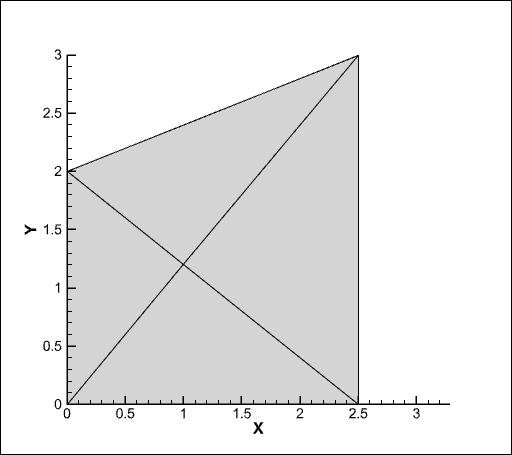
\includegraphics[width=0.75\textwidth]{mesh.png}
    \caption{分片实验网格}
\end{figure}
各节点的坐标、位移和载荷按照人工位移
$u_x(x,y) = 0.01x,\quad u_y(x,y) = -0.003y$计算如下表
\begin{table}[H]
\centering
\caption{各节点坐标、位移及载荷}
\begin{tabular}{|c|c|c|c|c|c|c|}
\hline
节点号 $I$ & $x_I$ & $y_I$ & $u_I$ & $v_I$ & $F_{xI}$ & $F_{yI}$ \\ 
\hline
1 & 0 & 0 & 0 & 0 & $-10$ & 0 \\ 
\hline
2 & 2.5 & 0 & 0.025 & 0 & 15 & 0 \\ 
\hline
3 & 2.5 & 3 & 0.025 & $-0.009$ & 10 & 0 \\ 
\hline
4 & 0 & 2 & 0 & $-0.006$ & $-15$ & 0 \\ 
\hline
5 & 1 & 1.2 & 0.01 & $-0.0036$ & 0 & 0 \\ 
\hline
\end{tabular}
\label{tab:node_data}
\end{table}

\subsubsection{A}
实验A要求将所有点位移给定,判断内部节点是否平衡,即节点力是否为零。输出结果如下
\begin{minted}{bash}
     N O D A L   F O R C E 
  NODE                        FX                FY                FZ
    1              -1.00000e+01       8.88178e-16       0.00000e+00
    2               1.50000e+01      -4.44089e-16       0.00000e+00
    3               1.00000e+01       1.77636e-15       0.00000e+00
    4              -1.50000e+01       8.88178e-16       0.00000e+00
    5              -1.55431e-15      -3.55271e-15       0.00000e+00
\end{minted}

内部节点节点5的节点力大小数量级为$10^{-15}$,在误差范围内,可视为达到平衡,通过
实验A。

\subsubsection{B}
实验B要求给定所有边界节点位移,计算内部节点位移是否与人工解相同。输出结果如下
\begin{minted}{bash}
     D I S P L A C E M E N T S
  NODE           X-DISPLACEMENT    Y-DISPLACEMENT    Z-DISPLACEMENT
    1               0.00000e+00       0.00000e+00       0.00000e+00
    2               2.50000e-02       0.00000e+00       0.00000e+00
    3               2.50000e-02      -9.00000e-03       0.00000e+00
    4               0.00000e+00      -6.00000e-03       0.00000e+00
    5               1.00000e-02      -3.60000e-03       0.00000e+00
\end{minted}

可见节点5的位移大小与人工解完全吻合。故通过分片实验B。

\subsubsection{C}
实验C仅仅施加最小限度的本质边界条件,同时再边界施加力条件,计算各个节点的解
是否与人工解相同。输出位移结果如下
\begin{minted}{bash}
     D I S P L A C E M E N T S
  NODE           X-DISPLACEMENT    Y-DISPLACEMENT    Z-DISPLACEMENT
    1               0.00000e+00       0.00000e+00       0.00000e+00
    2               2.50000e-02       0.00000e+00       0.00000e+00
    3               2.50000e-02      -9.00000e-03       0.00000e+00
    4               0.00000e+00      -6.00000e-03       0.00000e+00
    5               1.00000e-02      -3.60000e-03       0.00000e+00
\end{minted}

与人工解一致。实验C通过。

\subsection{收敛率分析}
参考教材习题4.12\cite{zhang2003},构造一个$L=10, h=2, b=1$的矩形截面悬臂梁,右端受力偶作用,且泊松比为零,模拟一维
应力状态。该情况下的解析解为
\begin{equation}
    u(x) = \frac{Fh}{EI}xy, \quad v(x) = -\frac{Fh}{2EI}x^2
\end{equation}

取$F=1, E=10000$。基础的网格划分如下图,即分成$N\times5N$个方形,每个方形斜向切分为两个三角形单元。
\begin{figure}[H]
    \centering
    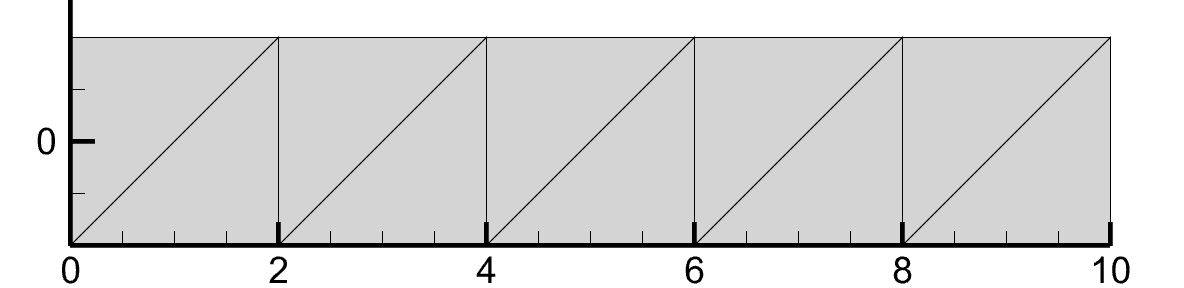
\includegraphics[width=0.75\textwidth]{mesh_1.png}
    \caption{收敛率分析的基础网格}
\end{figure}

以此类推,取$N=1,2,4,8$,分别计算解出单元的位移。其中$N=8$时利用Tecplot绘制的位移云图如下
\begin{figure}[H]
    \centering
    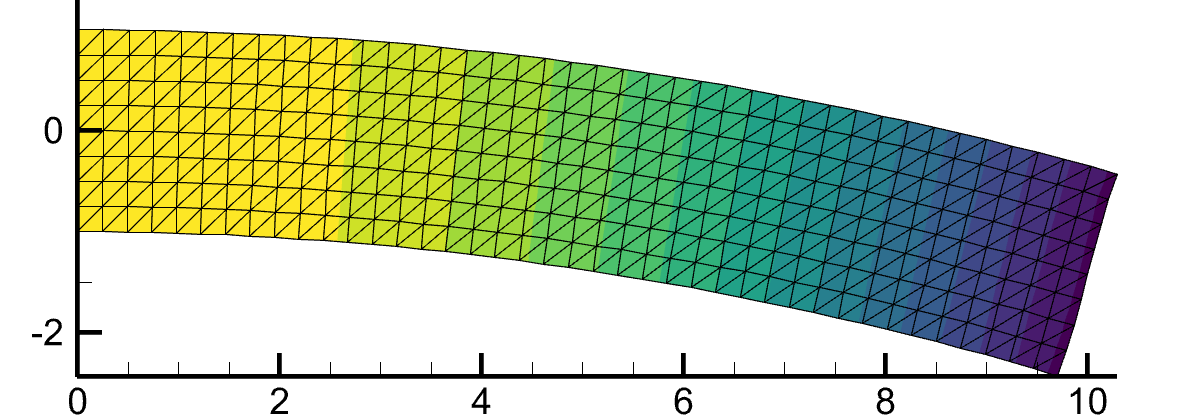
\includegraphics[width=0.75\textwidth]{cloud_map.png}
    \caption{$N=8$时的变形位移云图}
\end{figure}

对每一个$N$计算$L_2$误差范数。得到误差范数与单元尺寸双对数图如下
\begin{figure}[H]
    \centering
    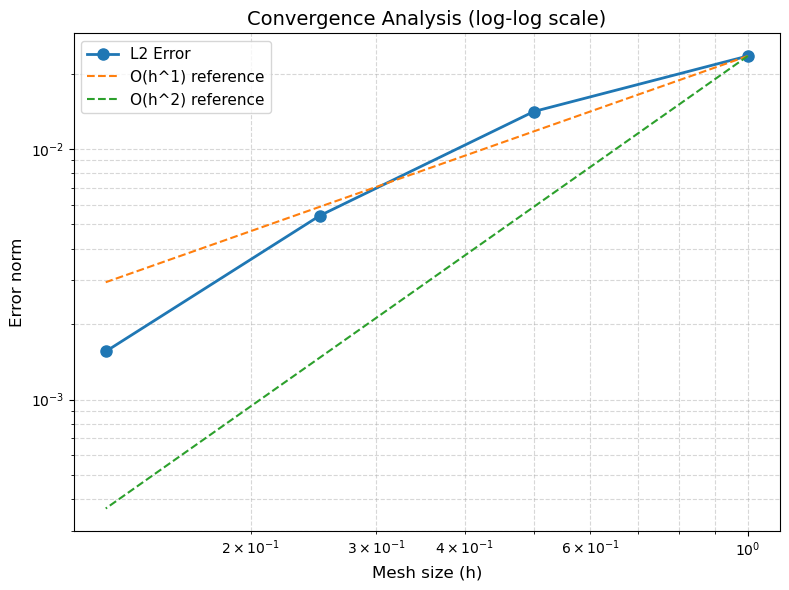
\includegraphics[width=0.75\textwidth]{log.png}
    \caption{位移的$L_2$误差范数与单元尺寸的双对数图}
\end{figure}

在单元尺寸较大时,因为此时的绝对误差大,故收敛速度慢;但是随着单元的加密
,误差的收敛速度渐进于$O(h^2)$,与理论分析吻合。

\subsection{验证算例}
此算例修改自教材习题4.12\cite{zhang2003}。在上表面施加均匀载荷$q=5000\mathrm{Pa}$,单元的弹性模量和泊松比
为$E=70\mathrm{GPa},\quad\nu=0.3$。

为了验证代码正确性和便于划分网格,在Abaqus软件上进行建模计算。然后将Abaqus的\code|inp|文件
中的网格信息导出并用脚本修改作为\code|STAPpp|的输入文件。该方法可以快速得到精密且复杂的网格,
省去了手动计算划分的时间,并保证Abaqus内的网格和验证计算文件的网格完全一致。

为了比较两者的结果,绘制拱桥右斜边的坐标——$X$位移曲线如下
\begin{figure}[H]
    \centering
    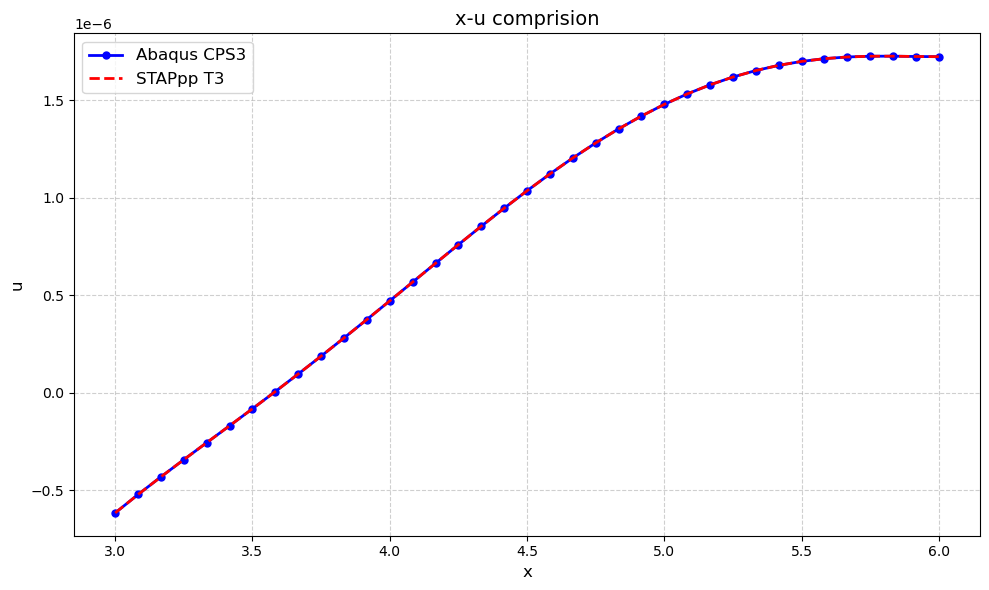
\includegraphics[width=0.5\textwidth]{comparison.png}
    \caption{拱桥算例的右斜边结果对比}
\end{figure}
两者的计算结果完全吻合,说明\code|STAPpp|的T3单元精度与Abaqus的
CPS3单元一致。

为了更加直观的观察形变结果,绘制位移云图如下
\begin{figure}[H]
    \centering
    \begin{subfigure}{0.6\textwidth}  % 调整宽度
        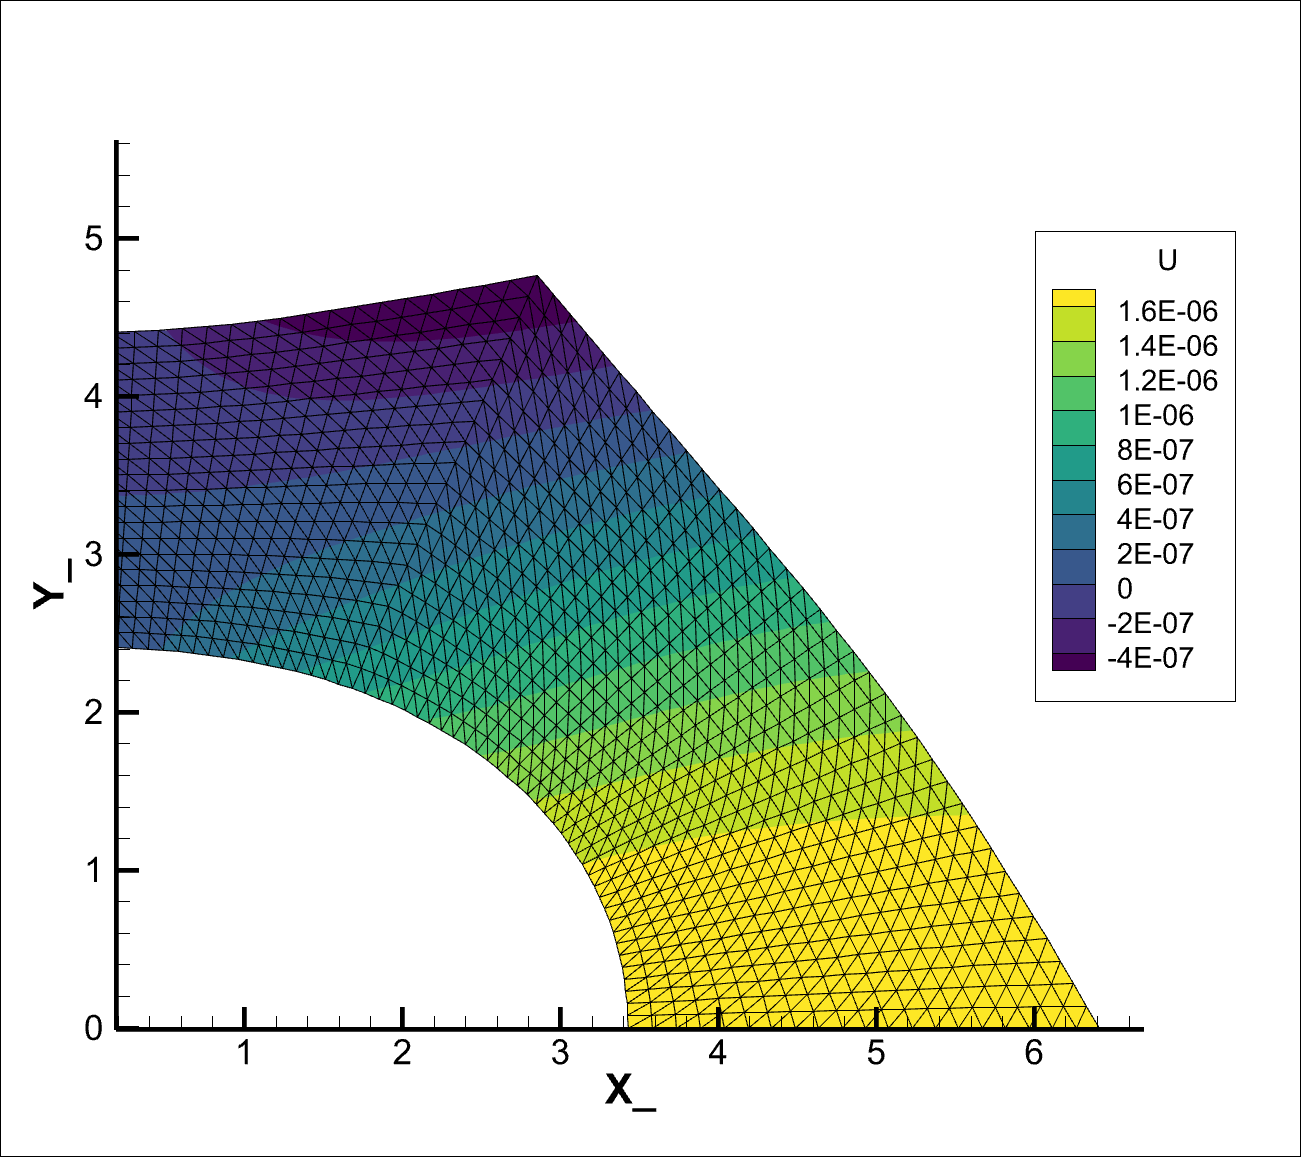
\includegraphics[width=\linewidth]{valiadtion.png}
        \caption{STAPpp结果}
        \label{fig:subfig1}
    \end{subfigure}
    \hfill  % 自动填充间距
    \begin{subfigure}{0.6\textwidth}
        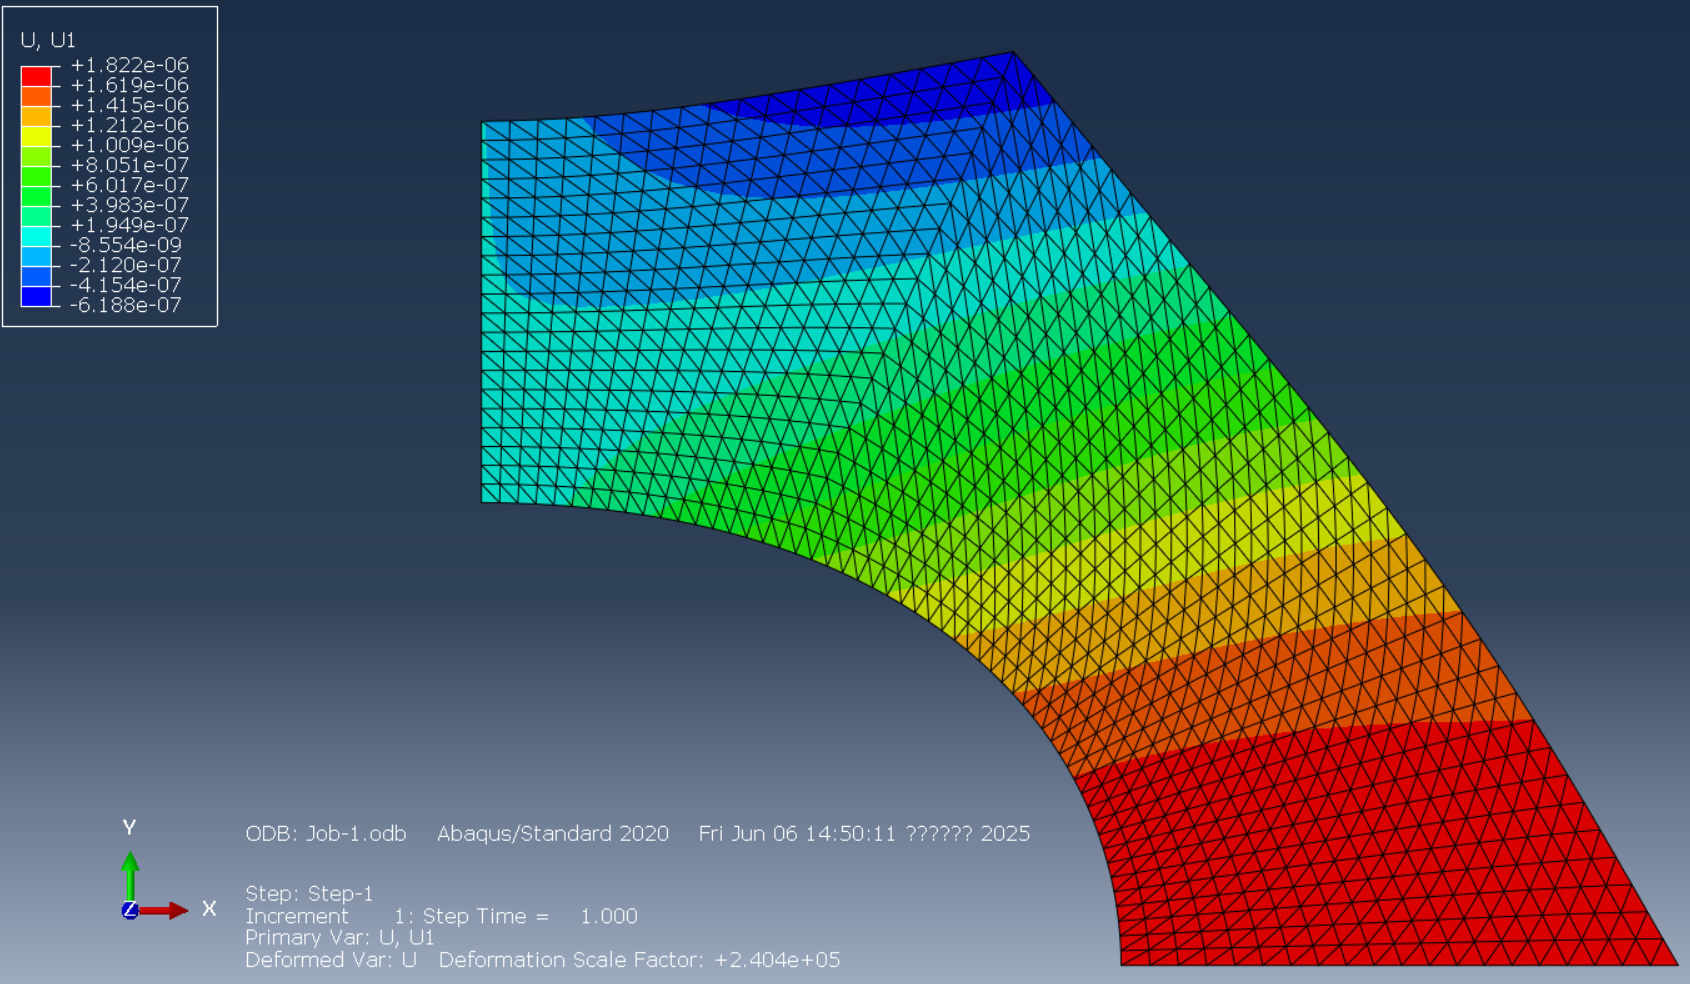
\includegraphics[width=\linewidth]{abaqus.png}
        \caption{Abaqus结果}
        \label{fig:subfig2}
    \end{subfigure}
    \caption{STAPpp位移云图与Abaqus位移云图对比(形变缩放比相同)}
\end{figure}

\section{任务分工与合作}
此次大作业由我独立完成。

\section{结论}
改进后的\code|STAPpp|程序能够正确计算T3单元的位移、节点力和单元应力,通过
分片实验、收敛分析和验证算例,证明了其分析平面应力问题的有效性和正确性。

\begin{thebibliography}{99}  % 99 是占位符,表示参考文献编号位数
\bibitem{zhang2003} 
张雄. 
\textbf{有限元法基础}. 
北京: 高等教育出版社, 2023.
\end{thebibliography}
\end{document}